\subsection*{Beregninger}

\begin{figure}[h]
\centering
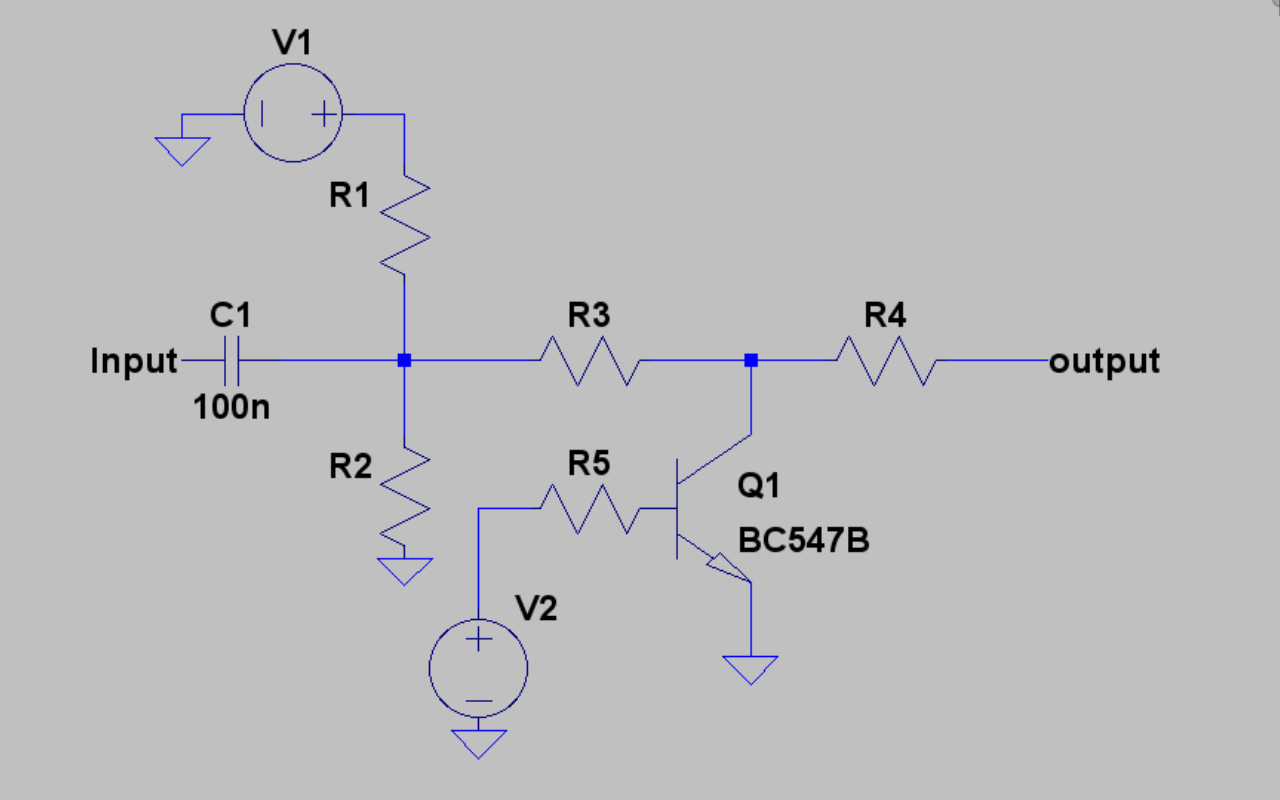
\includegraphics[scale=0.6]{implementering/indgangsvaelger/signal-taend-sluk.png}
\caption{Opbygning af indgangsvælgeren}
\label{indgangsvaelger-overordnet}
\end{figure}

Modstandene $R_1$ og $R_2$ er begge valgt til 100k\ohm, for at give et DC-offset på ca 2.5V, halvdelen af V1. Dette gælder dog kun når transistoren er slukket. I det transistoren tændes, sættes $R_2$ parallelt med $R_3$, hvilket trækker DC-offsettet længere ned:
\begin{equation}
5V\cdot \frac{\frac{1}{\frac{1}{R_2}+\frac{1}{R_3}}}{R_1+\frac{1}{\frac{1}{R_2}+\frac{1}{R_3}}}=1.11 V
\end{equation}
Dog er det egentlige DC-offset underordnet, så længe det ligger indenfor et område transistoren kan arbejde med, og DC-offset $-$ AC-Peakværdi $>$ 0 når transistoren er slukket. DC-offsettet alligevel bliver filtreret fra gennem en kondensator, før summationsforstærkeren, så det ikke har indflydelse på det endelige signal.
Modstanden $R_3$ er valgt ud fra, at signalet skal se en indgangsimpedans på minimum 22 k\ohm. Når transistoren er tændt er indgangsimpedansen mindst. $R_1$, $R_2$ og $R_3$ sidder så alle parallelt hvilket giver:
\begin{equation}
\frac{1}{\frac{1}{R_1}+\frac{1}{R_2}+\frac{1}{R_3}}=22 k\ohm
\\
R_3=39.29 k\ohm
\end{equation}
Denne er så valgt til 40.2k\ohm, for at passe med E96-rækken.
For at kunne afbryde de enkelte signaler, kan transistoren Q1 trække signalet til stel. for at tillade at hele signalet bliver trukket til stel, skal hele den strøm der løber igennem systemet føres ned igennem transistoren. Den maksimale strøm der kan løbe i systemet er summen af DC-strømmen og AC-strømmen. 
Først findes DC-strømmen. DC spændingen i kredsløbet er sat til 5V. Hvis transistoren en direkte kobling, så der ligger stel mellem $R_3$ og $R_4$, vil $R_2$ og $R_3$ sidde i parallel til stel. Ud fra dette findes den maksimale mængde strøm, der kan løbe igennem $R_3$. Ud fra dette den største strøm der vil løbe igennem $R_3$, og derfor også transistoren, udregnes til ca. 0.027 mA
Den maksimale AC-strøm findes ved at kortslutte alle kondensatorer, og regne med det størst mulige AC-udsving. En konsekvens af, at alle kondensatorer bliver kortsluttet, er at forsyning og stel også bliver kortsluttet. Ud fra dette findes AC-strømmen til at være ca. 0.05 mA. Dette giver en samlet max strøm på ca. 0.08 mA.
Strømmen $I_B$, som løber ind i basis på transistoren skal mindst være den samlede strøm, divideret med $H_{FE}$:
\begin{equation}
I_B = \frac{0.08 mA}{H_{FE}} = xx mA
\end{equation}
Da de benyttede flip-flops\fixme{Check at det stadig er sådan} outputter 5 V, kan $R_B$'s maksimale værdi findes:
\begin{equation}
R_B = \frac{5 V}{I_B} = xx k\ohm
\end{equation}
Alt under dette vil give en større strøm ind i basis, hvilket vil give en større strøm ind i collectorbenet og vil derfor også kunne trække signalet til stel.
Modstanden $R_4$ har ikke nogen indvirkning på indgangsimpedansen når transistoren er tændt og signalet derfor er slukket. Når signalet er tændt, sidder den i serie med $R_3$, hvilket giver en højere indgangsimpedans:
\begin{equation}
R_{indgang}=\frac{1}{\frac{1}{R_1}+\frac{1}{R_2}+\frac{1}{R_3+R_4}}=30.8 k\ohm
\end{equation}
$R_4$ er valgt til 40.2 k\ohm, det samme som $R_3$, for at gøre produceringen enklere. Ved at bruge modstande med de samme værdier sænkes antallet af benyttede komponenter, hvilket letter indkøbs- samt produceringsomkostninger \fixme{Skal der her skrottes? Kunne virkelig godt tænke mig at vi fandt en grund til at værdien skal være som den er.}.
Efter at have opstillet de forskellige modstandsværdier, er det muligt at udregne værdien af afkoblingskondensatorerne i kredsløbet. Disse kan udregnes som en spændingsdeling mellem en seriekoblet modstand og kondensator, seriekoblet med en modstand, som vist på figur \ref{crvd}. I dette tilfælde vil $R_U$ være udgangsimpedansen på det foregående led, og $R_I$ være indgangsimpedansen på det efterfølgende. Impedansen i en kondensator, i frekvensdomænet er $\frac{1}{s\cdot C}$. Dette kan opstilles i følge spændingsdelingsformel for udregningen:
\begin{equation}
\frac{V_{out}}{V_{in}}=\frac{R_I}{R_I+(R_U+\frac{1}{s\cdot C})}
\end{equation}
For at få en dæmpning på 3dB, som er den ønskede dæmpning i knækpunktet, skal $\frac{V_{out}}{V_{in}}=10^{\frac{-3}{20}}\approx0.7$. 
Dette giver 2 ubekendte, s og C. s kan ses som $2\cdot \pi \cdot f$, hvor f er den ønskede frekvens ved knækket. Der opstilles et udtryk for C:
\begin{equation}
10^{\frac{-3}{20}}=\frac{R_I}{R_I+(R_U+\frac{1}{2\cdot\pi\cdot 2\cdot C})}\\
C=\frac{-1}{2}\cdot{10^{\frac{-3}{20}}}{\pi\cdot f\cdot(10^{\frac{-3}{20}}\cdot R_I+\frac{-3}{20}}\cdot R_U - R_I)
\end{equation}
f bestemmes til 2hz, én dekade før den ønskede, for at opnå en lav dæmpning ved de ønskede 20hz. Ud fra dette kan de forskellige værdier for C udregnes, afhængigt af de impedanser de ser ind i.
Indgangsimpedansen for $C_1$ er fundet til 30.8 k\ohm . Indtastes dette i ovennævnte formel findes værdien for $C_1$ til mindst 8µF. Alt under dette vil give en højere knækfrekvens, hvilket ikke er at ønske. Alt højere vil dog give en større indsvingningstid, hvilket er at foretrække, dog heller ikke ønskeligt.